
% Default to the notebook output style

    


% Inherit from the specified cell style.




    
\documentclass[11pt]{article}

    
    
    \usepackage[T1]{fontenc}
    % Nicer default font (+ math font) than Computer Modern for most use cases
    \usepackage{mathpazo}

    % Basic figure setup, for now with no caption control since it's done
    % automatically by Pandoc (which extracts ![](path) syntax from Markdown).
    \usepackage{graphicx}
    % We will generate all images so they have a width \maxwidth. This means
    % that they will get their normal width if they fit onto the page, but
    % are scaled down if they would overflow the margins.
    \makeatletter
    \def\maxwidth{\ifdim\Gin@nat@width>\linewidth\linewidth
    \else\Gin@nat@width\fi}
    \makeatother
    \let\Oldincludegraphics\includegraphics
    % Set max figure width to be 80% of text width, for now hardcoded.
    \renewcommand{\includegraphics}[1]{\Oldincludegraphics[width=.8\maxwidth]{#1}}
    % Ensure that by default, figures have no caption (until we provide a
    % proper Figure object with a Caption API and a way to capture that
    % in the conversion process - todo).
    \usepackage{caption}
    \DeclareCaptionLabelFormat{nolabel}{}
    \captionsetup{labelformat=nolabel}

    \usepackage{adjustbox} % Used to constrain images to a maximum size 
    \usepackage{xcolor} % Allow colors to be defined
    \usepackage{enumerate} % Needed for markdown enumerations to work
    \usepackage{geometry} % Used to adjust the document margins
    \usepackage{amsmath} % Equations
    \usepackage{amssymb} % Equations
    \usepackage{textcomp} % defines textquotesingle
    % Hack from http://tex.stackexchange.com/a/47451/13684:
    \AtBeginDocument{%
        \def\PYZsq{\textquotesingle}% Upright quotes in Pygmentized code
    }
    \usepackage{upquote} % Upright quotes for verbatim code
    \usepackage{eurosym} % defines \euro
    \usepackage[mathletters]{ucs} % Extended unicode (utf-8) support
    \usepackage[utf8x]{inputenc} % Allow utf-8 characters in the tex document
    \usepackage{fancyvrb} % verbatim replacement that allows latex
    \usepackage{grffile} % extends the file name processing of package graphics 
                         % to support a larger range 
    % The hyperref package gives us a pdf with properly built
    % internal navigation ('pdf bookmarks' for the table of contents,
    % internal cross-reference links, web links for URLs, etc.)
    \usepackage{hyperref}
    \usepackage{longtable} % longtable support required by pandoc >1.10
    \usepackage{booktabs}  % table support for pandoc > 1.12.2
    \usepackage[inline]{enumitem} % IRkernel/repr support (it uses the enumerate* environment)
    \usepackage[normalem]{ulem} % ulem is needed to support strikethroughs (\sout)
                                % normalem makes italics be italics, not underlines
    

    
    
    % Colors for the hyperref package
    \definecolor{urlcolor}{rgb}{0,.145,.698}
    \definecolor{linkcolor}{rgb}{.71,0.21,0.01}
    \definecolor{citecolor}{rgb}{.12,.54,.11}

    % ANSI colors
    \definecolor{ansi-black}{HTML}{3E424D}
    \definecolor{ansi-black-intense}{HTML}{282C36}
    \definecolor{ansi-red}{HTML}{E75C58}
    \definecolor{ansi-red-intense}{HTML}{B22B31}
    \definecolor{ansi-green}{HTML}{00A250}
    \definecolor{ansi-green-intense}{HTML}{007427}
    \definecolor{ansi-yellow}{HTML}{DDB62B}
    \definecolor{ansi-yellow-intense}{HTML}{B27D12}
    \definecolor{ansi-blue}{HTML}{208FFB}
    \definecolor{ansi-blue-intense}{HTML}{0065CA}
    \definecolor{ansi-magenta}{HTML}{D160C4}
    \definecolor{ansi-magenta-intense}{HTML}{A03196}
    \definecolor{ansi-cyan}{HTML}{60C6C8}
    \definecolor{ansi-cyan-intense}{HTML}{258F8F}
    \definecolor{ansi-white}{HTML}{C5C1B4}
    \definecolor{ansi-white-intense}{HTML}{A1A6B2}

    % commands and environments needed by pandoc snippets
    % extracted from the output of `pandoc -s`
    \providecommand{\tightlist}{%
      \setlength{\itemsep}{0pt}\setlength{\parskip}{0pt}}
    \DefineVerbatimEnvironment{Highlighting}{Verbatim}{commandchars=\\\{\}}
    % Add ',fontsize=\small' for more characters per line
    \newenvironment{Shaded}{}{}
    \newcommand{\KeywordTok}[1]{\textcolor[rgb]{0.00,0.44,0.13}{\textbf{{#1}}}}
    \newcommand{\DataTypeTok}[1]{\textcolor[rgb]{0.56,0.13,0.00}{{#1}}}
    \newcommand{\DecValTok}[1]{\textcolor[rgb]{0.25,0.63,0.44}{{#1}}}
    \newcommand{\BaseNTok}[1]{\textcolor[rgb]{0.25,0.63,0.44}{{#1}}}
    \newcommand{\FloatTok}[1]{\textcolor[rgb]{0.25,0.63,0.44}{{#1}}}
    \newcommand{\CharTok}[1]{\textcolor[rgb]{0.25,0.44,0.63}{{#1}}}
    \newcommand{\StringTok}[1]{\textcolor[rgb]{0.25,0.44,0.63}{{#1}}}
    \newcommand{\CommentTok}[1]{\textcolor[rgb]{0.38,0.63,0.69}{\textit{{#1}}}}
    \newcommand{\OtherTok}[1]{\textcolor[rgb]{0.00,0.44,0.13}{{#1}}}
    \newcommand{\AlertTok}[1]{\textcolor[rgb]{1.00,0.00,0.00}{\textbf{{#1}}}}
    \newcommand{\FunctionTok}[1]{\textcolor[rgb]{0.02,0.16,0.49}{{#1}}}
    \newcommand{\RegionMarkerTok}[1]{{#1}}
    \newcommand{\ErrorTok}[1]{\textcolor[rgb]{1.00,0.00,0.00}{\textbf{{#1}}}}
    \newcommand{\NormalTok}[1]{{#1}}
    
    % Additional commands for more recent versions of Pandoc
    \newcommand{\ConstantTok}[1]{\textcolor[rgb]{0.53,0.00,0.00}{{#1}}}
    \newcommand{\SpecialCharTok}[1]{\textcolor[rgb]{0.25,0.44,0.63}{{#1}}}
    \newcommand{\VerbatimStringTok}[1]{\textcolor[rgb]{0.25,0.44,0.63}{{#1}}}
    \newcommand{\SpecialStringTok}[1]{\textcolor[rgb]{0.73,0.40,0.53}{{#1}}}
    \newcommand{\ImportTok}[1]{{#1}}
    \newcommand{\DocumentationTok}[1]{\textcolor[rgb]{0.73,0.13,0.13}{\textit{{#1}}}}
    \newcommand{\AnnotationTok}[1]{\textcolor[rgb]{0.38,0.63,0.69}{\textbf{\textit{{#1}}}}}
    \newcommand{\CommentVarTok}[1]{\textcolor[rgb]{0.38,0.63,0.69}{\textbf{\textit{{#1}}}}}
    \newcommand{\VariableTok}[1]{\textcolor[rgb]{0.10,0.09,0.49}{{#1}}}
    \newcommand{\ControlFlowTok}[1]{\textcolor[rgb]{0.00,0.44,0.13}{\textbf{{#1}}}}
    \newcommand{\OperatorTok}[1]{\textcolor[rgb]{0.40,0.40,0.40}{{#1}}}
    \newcommand{\BuiltInTok}[1]{{#1}}
    \newcommand{\ExtensionTok}[1]{{#1}}
    \newcommand{\PreprocessorTok}[1]{\textcolor[rgb]{0.74,0.48,0.00}{{#1}}}
    \newcommand{\AttributeTok}[1]{\textcolor[rgb]{0.49,0.56,0.16}{{#1}}}
    \newcommand{\InformationTok}[1]{\textcolor[rgb]{0.38,0.63,0.69}{\textbf{\textit{{#1}}}}}
    \newcommand{\WarningTok}[1]{\textcolor[rgb]{0.38,0.63,0.69}{\textbf{\textit{{#1}}}}}
    
    
    % Define a nice break command that doesn't care if a line doesn't already
    % exist.
    \def\br{\hspace*{\fill} \\* }
    % Math Jax compatability definitions
    \def\gt{>}
    \def\lt{<}
    % Document parameters
    \title{hw3-svm}
    
    
    

    % Pygments definitions
    
\makeatletter
\def\PY@reset{\let\PY@it=\relax \let\PY@bf=\relax%
    \let\PY@ul=\relax \let\PY@tc=\relax%
    \let\PY@bc=\relax \let\PY@ff=\relax}
\def\PY@tok#1{\csname PY@tok@#1\endcsname}
\def\PY@toks#1+{\ifx\relax#1\empty\else%
    \PY@tok{#1}\expandafter\PY@toks\fi}
\def\PY@do#1{\PY@bc{\PY@tc{\PY@ul{%
    \PY@it{\PY@bf{\PY@ff{#1}}}}}}}
\def\PY#1#2{\PY@reset\PY@toks#1+\relax+\PY@do{#2}}

\expandafter\def\csname PY@tok@w\endcsname{\def\PY@tc##1{\textcolor[rgb]{0.73,0.73,0.73}{##1}}}
\expandafter\def\csname PY@tok@c\endcsname{\let\PY@it=\textit\def\PY@tc##1{\textcolor[rgb]{0.25,0.50,0.50}{##1}}}
\expandafter\def\csname PY@tok@cp\endcsname{\def\PY@tc##1{\textcolor[rgb]{0.74,0.48,0.00}{##1}}}
\expandafter\def\csname PY@tok@k\endcsname{\let\PY@bf=\textbf\def\PY@tc##1{\textcolor[rgb]{0.00,0.50,0.00}{##1}}}
\expandafter\def\csname PY@tok@kp\endcsname{\def\PY@tc##1{\textcolor[rgb]{0.00,0.50,0.00}{##1}}}
\expandafter\def\csname PY@tok@kt\endcsname{\def\PY@tc##1{\textcolor[rgb]{0.69,0.00,0.25}{##1}}}
\expandafter\def\csname PY@tok@o\endcsname{\def\PY@tc##1{\textcolor[rgb]{0.40,0.40,0.40}{##1}}}
\expandafter\def\csname PY@tok@ow\endcsname{\let\PY@bf=\textbf\def\PY@tc##1{\textcolor[rgb]{0.67,0.13,1.00}{##1}}}
\expandafter\def\csname PY@tok@nb\endcsname{\def\PY@tc##1{\textcolor[rgb]{0.00,0.50,0.00}{##1}}}
\expandafter\def\csname PY@tok@nf\endcsname{\def\PY@tc##1{\textcolor[rgb]{0.00,0.00,1.00}{##1}}}
\expandafter\def\csname PY@tok@nc\endcsname{\let\PY@bf=\textbf\def\PY@tc##1{\textcolor[rgb]{0.00,0.00,1.00}{##1}}}
\expandafter\def\csname PY@tok@nn\endcsname{\let\PY@bf=\textbf\def\PY@tc##1{\textcolor[rgb]{0.00,0.00,1.00}{##1}}}
\expandafter\def\csname PY@tok@ne\endcsname{\let\PY@bf=\textbf\def\PY@tc##1{\textcolor[rgb]{0.82,0.25,0.23}{##1}}}
\expandafter\def\csname PY@tok@nv\endcsname{\def\PY@tc##1{\textcolor[rgb]{0.10,0.09,0.49}{##1}}}
\expandafter\def\csname PY@tok@no\endcsname{\def\PY@tc##1{\textcolor[rgb]{0.53,0.00,0.00}{##1}}}
\expandafter\def\csname PY@tok@nl\endcsname{\def\PY@tc##1{\textcolor[rgb]{0.63,0.63,0.00}{##1}}}
\expandafter\def\csname PY@tok@ni\endcsname{\let\PY@bf=\textbf\def\PY@tc##1{\textcolor[rgb]{0.60,0.60,0.60}{##1}}}
\expandafter\def\csname PY@tok@na\endcsname{\def\PY@tc##1{\textcolor[rgb]{0.49,0.56,0.16}{##1}}}
\expandafter\def\csname PY@tok@nt\endcsname{\let\PY@bf=\textbf\def\PY@tc##1{\textcolor[rgb]{0.00,0.50,0.00}{##1}}}
\expandafter\def\csname PY@tok@nd\endcsname{\def\PY@tc##1{\textcolor[rgb]{0.67,0.13,1.00}{##1}}}
\expandafter\def\csname PY@tok@s\endcsname{\def\PY@tc##1{\textcolor[rgb]{0.73,0.13,0.13}{##1}}}
\expandafter\def\csname PY@tok@sd\endcsname{\let\PY@it=\textit\def\PY@tc##1{\textcolor[rgb]{0.73,0.13,0.13}{##1}}}
\expandafter\def\csname PY@tok@si\endcsname{\let\PY@bf=\textbf\def\PY@tc##1{\textcolor[rgb]{0.73,0.40,0.53}{##1}}}
\expandafter\def\csname PY@tok@se\endcsname{\let\PY@bf=\textbf\def\PY@tc##1{\textcolor[rgb]{0.73,0.40,0.13}{##1}}}
\expandafter\def\csname PY@tok@sr\endcsname{\def\PY@tc##1{\textcolor[rgb]{0.73,0.40,0.53}{##1}}}
\expandafter\def\csname PY@tok@ss\endcsname{\def\PY@tc##1{\textcolor[rgb]{0.10,0.09,0.49}{##1}}}
\expandafter\def\csname PY@tok@sx\endcsname{\def\PY@tc##1{\textcolor[rgb]{0.00,0.50,0.00}{##1}}}
\expandafter\def\csname PY@tok@m\endcsname{\def\PY@tc##1{\textcolor[rgb]{0.40,0.40,0.40}{##1}}}
\expandafter\def\csname PY@tok@gh\endcsname{\let\PY@bf=\textbf\def\PY@tc##1{\textcolor[rgb]{0.00,0.00,0.50}{##1}}}
\expandafter\def\csname PY@tok@gu\endcsname{\let\PY@bf=\textbf\def\PY@tc##1{\textcolor[rgb]{0.50,0.00,0.50}{##1}}}
\expandafter\def\csname PY@tok@gd\endcsname{\def\PY@tc##1{\textcolor[rgb]{0.63,0.00,0.00}{##1}}}
\expandafter\def\csname PY@tok@gi\endcsname{\def\PY@tc##1{\textcolor[rgb]{0.00,0.63,0.00}{##1}}}
\expandafter\def\csname PY@tok@gr\endcsname{\def\PY@tc##1{\textcolor[rgb]{1.00,0.00,0.00}{##1}}}
\expandafter\def\csname PY@tok@ge\endcsname{\let\PY@it=\textit}
\expandafter\def\csname PY@tok@gs\endcsname{\let\PY@bf=\textbf}
\expandafter\def\csname PY@tok@gp\endcsname{\let\PY@bf=\textbf\def\PY@tc##1{\textcolor[rgb]{0.00,0.00,0.50}{##1}}}
\expandafter\def\csname PY@tok@go\endcsname{\def\PY@tc##1{\textcolor[rgb]{0.53,0.53,0.53}{##1}}}
\expandafter\def\csname PY@tok@gt\endcsname{\def\PY@tc##1{\textcolor[rgb]{0.00,0.27,0.87}{##1}}}
\expandafter\def\csname PY@tok@err\endcsname{\def\PY@bc##1{\setlength{\fboxsep}{0pt}\fcolorbox[rgb]{1.00,0.00,0.00}{1,1,1}{\strut ##1}}}
\expandafter\def\csname PY@tok@kc\endcsname{\let\PY@bf=\textbf\def\PY@tc##1{\textcolor[rgb]{0.00,0.50,0.00}{##1}}}
\expandafter\def\csname PY@tok@kd\endcsname{\let\PY@bf=\textbf\def\PY@tc##1{\textcolor[rgb]{0.00,0.50,0.00}{##1}}}
\expandafter\def\csname PY@tok@kn\endcsname{\let\PY@bf=\textbf\def\PY@tc##1{\textcolor[rgb]{0.00,0.50,0.00}{##1}}}
\expandafter\def\csname PY@tok@kr\endcsname{\let\PY@bf=\textbf\def\PY@tc##1{\textcolor[rgb]{0.00,0.50,0.00}{##1}}}
\expandafter\def\csname PY@tok@bp\endcsname{\def\PY@tc##1{\textcolor[rgb]{0.00,0.50,0.00}{##1}}}
\expandafter\def\csname PY@tok@fm\endcsname{\def\PY@tc##1{\textcolor[rgb]{0.00,0.00,1.00}{##1}}}
\expandafter\def\csname PY@tok@vc\endcsname{\def\PY@tc##1{\textcolor[rgb]{0.10,0.09,0.49}{##1}}}
\expandafter\def\csname PY@tok@vg\endcsname{\def\PY@tc##1{\textcolor[rgb]{0.10,0.09,0.49}{##1}}}
\expandafter\def\csname PY@tok@vi\endcsname{\def\PY@tc##1{\textcolor[rgb]{0.10,0.09,0.49}{##1}}}
\expandafter\def\csname PY@tok@vm\endcsname{\def\PY@tc##1{\textcolor[rgb]{0.10,0.09,0.49}{##1}}}
\expandafter\def\csname PY@tok@sa\endcsname{\def\PY@tc##1{\textcolor[rgb]{0.73,0.13,0.13}{##1}}}
\expandafter\def\csname PY@tok@sb\endcsname{\def\PY@tc##1{\textcolor[rgb]{0.73,0.13,0.13}{##1}}}
\expandafter\def\csname PY@tok@sc\endcsname{\def\PY@tc##1{\textcolor[rgb]{0.73,0.13,0.13}{##1}}}
\expandafter\def\csname PY@tok@dl\endcsname{\def\PY@tc##1{\textcolor[rgb]{0.73,0.13,0.13}{##1}}}
\expandafter\def\csname PY@tok@s2\endcsname{\def\PY@tc##1{\textcolor[rgb]{0.73,0.13,0.13}{##1}}}
\expandafter\def\csname PY@tok@sh\endcsname{\def\PY@tc##1{\textcolor[rgb]{0.73,0.13,0.13}{##1}}}
\expandafter\def\csname PY@tok@s1\endcsname{\def\PY@tc##1{\textcolor[rgb]{0.73,0.13,0.13}{##1}}}
\expandafter\def\csname PY@tok@mb\endcsname{\def\PY@tc##1{\textcolor[rgb]{0.40,0.40,0.40}{##1}}}
\expandafter\def\csname PY@tok@mf\endcsname{\def\PY@tc##1{\textcolor[rgb]{0.40,0.40,0.40}{##1}}}
\expandafter\def\csname PY@tok@mh\endcsname{\def\PY@tc##1{\textcolor[rgb]{0.40,0.40,0.40}{##1}}}
\expandafter\def\csname PY@tok@mi\endcsname{\def\PY@tc##1{\textcolor[rgb]{0.40,0.40,0.40}{##1}}}
\expandafter\def\csname PY@tok@il\endcsname{\def\PY@tc##1{\textcolor[rgb]{0.40,0.40,0.40}{##1}}}
\expandafter\def\csname PY@tok@mo\endcsname{\def\PY@tc##1{\textcolor[rgb]{0.40,0.40,0.40}{##1}}}
\expandafter\def\csname PY@tok@ch\endcsname{\let\PY@it=\textit\def\PY@tc##1{\textcolor[rgb]{0.25,0.50,0.50}{##1}}}
\expandafter\def\csname PY@tok@cm\endcsname{\let\PY@it=\textit\def\PY@tc##1{\textcolor[rgb]{0.25,0.50,0.50}{##1}}}
\expandafter\def\csname PY@tok@cpf\endcsname{\let\PY@it=\textit\def\PY@tc##1{\textcolor[rgb]{0.25,0.50,0.50}{##1}}}
\expandafter\def\csname PY@tok@c1\endcsname{\let\PY@it=\textit\def\PY@tc##1{\textcolor[rgb]{0.25,0.50,0.50}{##1}}}
\expandafter\def\csname PY@tok@cs\endcsname{\let\PY@it=\textit\def\PY@tc##1{\textcolor[rgb]{0.25,0.50,0.50}{##1}}}

\def\PYZbs{\char`\\}
\def\PYZus{\char`\_}
\def\PYZob{\char`\{}
\def\PYZcb{\char`\}}
\def\PYZca{\char`\^}
\def\PYZam{\char`\&}
\def\PYZlt{\char`\<}
\def\PYZgt{\char`\>}
\def\PYZsh{\char`\#}
\def\PYZpc{\char`\%}
\def\PYZdl{\char`\$}
\def\PYZhy{\char`\-}
\def\PYZsq{\char`\'}
\def\PYZdq{\char`\"}
\def\PYZti{\char`\~}
% for compatibility with earlier versions
\def\PYZat{@}
\def\PYZlb{[}
\def\PYZrb{]}
\makeatother


    % Exact colors from NB
    \definecolor{incolor}{rgb}{0.0, 0.0, 0.5}
    \definecolor{outcolor}{rgb}{0.545, 0.0, 0.0}



    
    % Prevent overflowing lines due to hard-to-break entities
    \sloppy 
    % Setup hyperref package
    \hypersetup{
      breaklinks=true,  % so long urls are correctly broken across lines
      colorlinks=true,
      urlcolor=urlcolor,
      linkcolor=linkcolor,
      citecolor=citecolor,
      }
    % Slightly bigger margins than the latex defaults
    
    \geometry{verbose,tmargin=1in,bmargin=1in,lmargin=1in,rmargin=1in}
    
    

    \begin{document}
    
    
    \maketitle
    
    

    
    \hypertarget{homework-3-svm-and-sentiment-analysis}{%
\section{Homework 3: SVM and Sentiment
Analysis}\label{homework-3-svm-and-sentiment-analysis}}

    \hypertarget{introduction}{%
\subsection{1 Introduction}\label{introduction}}

In this assignment, we'll be working with natural language data. In
particular, we'll be doing sentiment analysis on movie reviews. This
problem will give you the opportunity to try your hand at feature
engineering, which is one of the most important parts of many data
science problems. From a technical standpoint, this homework has two new
pieces. First, you'll be implementing Pegasos. Pegasos is essentially
stochastic subgradient descent for the SVM with a particular schedule
for the step-size. Second, because in natural langauge domains we
typically have huge feature spaces, we work with sparse representations
of feature vectors, where only the non-zero entries are explicitly
recorded. This will require coding your gradient and SGD code using hash
tables (dictionaries in Python), rather than numpy arrays. We begin with
some practice with subgradients and an easy problem that introduces the
Perceptron algorithm.

    \hypertarget{calculating-subgradients}{%
\subsection{2 Calculating Subgradients}\label{calculating-subgradients}}

Recall that a vector \(g\in\Re^{d}\) is a \(\textbf{subgradient}\) of
\(f:\Re^{d}\to\Re\) at \(x\) if for all \(z\), \[
f(z)\ge f(x)+g^{T}(z-x).
\] As we noted in lecture, there may be \(0\), \(1\), or infinitely many
subgradients at any point. The \(\textbf{subdifferential}\) of \(f\) at
a point \(x\), denoted \(\partial f(x)\), is the set of all subgradients
of \(f\) at \(x\).

    \begin{enumerate}
\def\labelenumi{\arabic{enumi}.}
\tightlist
\item
  Subgradients for pointwise maximum of functions. Suppose
  \(f_{1},\ldots,f_{m}:\Re^{d}\to\Re\) are convex functions, and
\end{enumerate}

\[
f(x)=\max_{i=1,\ldots,,m}f_{i}(x).
\]

Let \(k\) be any index for which \(f_{k}(x)=f(x)\), and choose
\(g\in\partial f_{k}(x)\). We are using the fact that a convex function
on \(\Re^{d}\) has a non-empty subdifferential at all points. Show that
\(g\in\partial f(x)\).

    \textbf{Answer}: We can find \(f(x) = f_{k}(x)\) for any exsiting \(k\),
let \(g\in\partial f_{k}(x)\) at point \(x\), and any
\(f_k(z)\ge f_k(x)+g^{T}(z-x)\), so
\(f(z) \ge f_k(z) \ge f_k(x)+g^{T}(z-x)\), so \(g\) must be
\(g\in\partial f(x)\).

    \begin{enumerate}
\def\labelenumi{\arabic{enumi}.}
\setcounter{enumi}{1}
\tightlist
\item
  Subgradient of hinge loss for linear prediction. Give a subgradient of
\end{enumerate}

\[
J(w)=\max\left\{ 0,1-yw^{T}x\right\} .
\]

    \textbf{Answer}: compute the subgradient of hinge loss function \[
\partial J(w)= 
\begin{cases}
  -1 & \text{if $yw^{T}x < 1$} \\
  0 & \text{if $yw^{T}x > 1$} \\
  [-1,0] & \text{if $yw^{T}x = 1$}
\end{cases}.
\]

    \hypertarget{perceptron}{%
\subsection{3 Perceptron}\label{perceptron}}

The perceptron algorithm is often the first classification algorithm
taught in machine learning classes. Suppose we have a labeled training
set
\$\left(x\_\{1\},y\_\{1\}\right),\ldots,(x\_\{n\},y\_\{n\})\in\Re\^{}\{d\}\times\left\{
-1,1\right\} \$. In the perceptron algorithm, we are looking for a
hyperplane that perfectly separates the classes. That is, we're looking
for \(w\in\Re^{d}\) such that

\[
y_{i}w^{T}x_{i}>0\;\forall i\in\left\{ 1,\ldots,n\right\} .
\]

Visually, this would mean that all the \(x\)'s with label \(y=1\) are on
one side of the hyperplane \$\left\{ x\mid w\^{}\{T\}x=0\right\} \$, and
all the \(x's\) with label \(y=-1\) are on the other side. When such a
hyperplane exists, we say that the data are
\(\textbf{linearly separable}\). The perceptron algorithm is given in
Algorithm 1 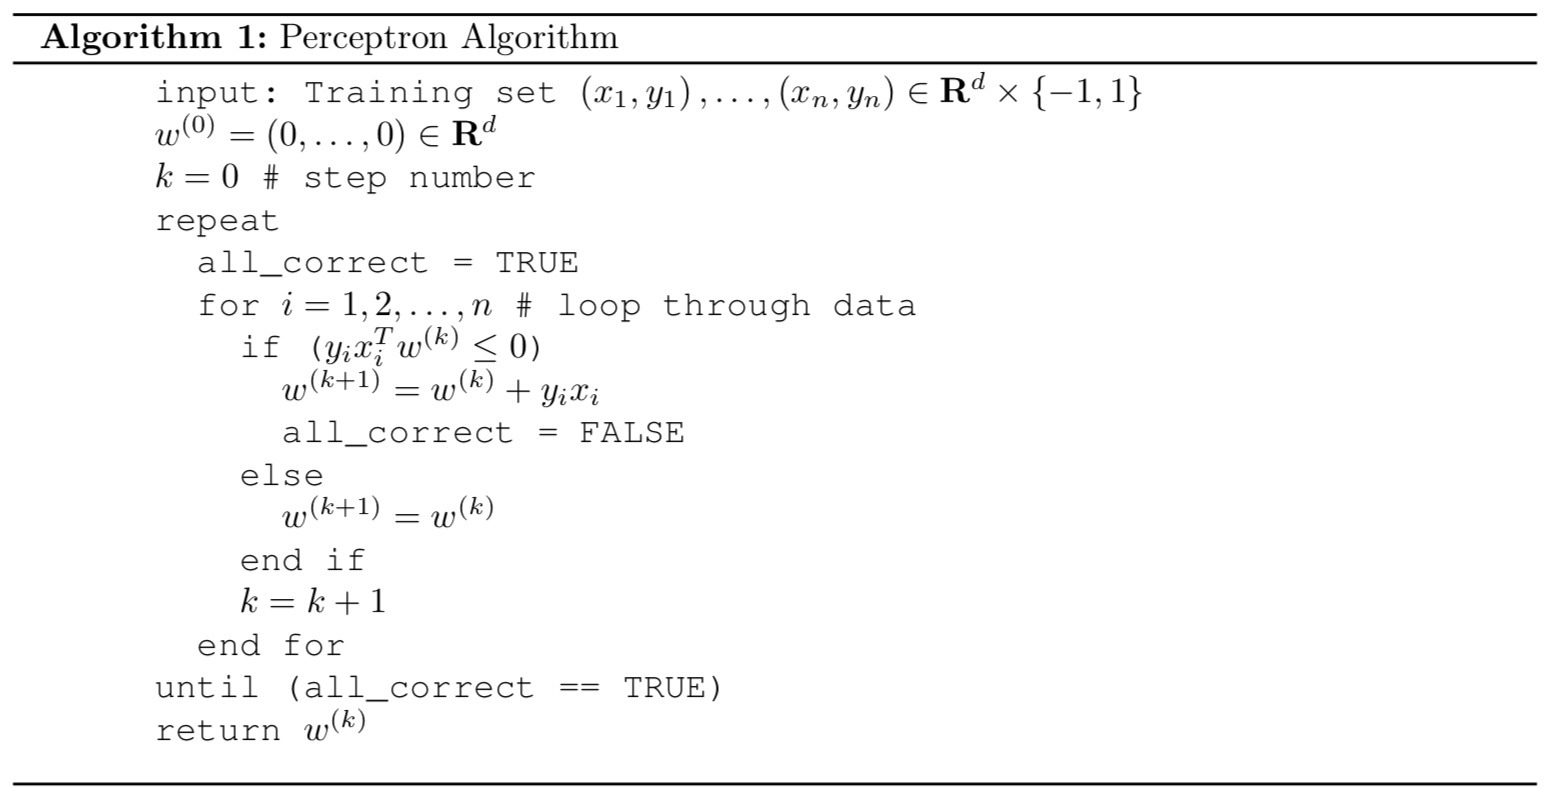
\includegraphics{perceptron.png}.

There is also something called the \(\textbf{perceptron loss,}\) given
by

\[
\ell(\hat{y},y)=\max\left\{ 0,-\hat{y}y\right\} .
\]

    \begin{enumerate}
\def\labelenumi{\arabic{enumi}.}
\tightlist
\item
  Show that if \$\left\{ x\mid w\^{}\{T\}x=0\right\} \$ is a separating
  hyperplane for a training set
  \(D=\left(\left(x_{1},y_{1}\right),\ldots,(x_{n},y_{n})\right)\), then
  the average perceptron loss on \(D\) is \(0\). Thus any separating
  hyperplane of \(D\) is an empirical risk minimizer for perceptron
  loss.
\end{enumerate}

    \textbf{Answer}: if \$\left\{ x\mid w\^{}\{T\}x=0\right\} \$ is a
separating hyperplane for a training set
\(D=\left(\left(x_{1},y_{1}\right),\ldots,(x_{n},y_{n})\right)\), we
always have
\(y_{i}w^{T}x_{i}>0\;\forall i\in\left\{ 1,\ldots,n\right\}\), which
means that \(\hat{y}y > 0\) always. Then the perceptron loss for each
training example is \(0\).

    \begin{enumerate}
\def\labelenumi{\arabic{enumi}.}
\setcounter{enumi}{1}
\tightlist
\item
  Let \(H\) be the linear hypothesis space consisting of functions
  \(x\mapsto w^{T}x\). Consider running stochastic subgradient descent
  (SSGD) to minimize the empirical risk with the perceptron loss. We'll
  use the version of SSGD in which we cycle through the data points in
  each epoch. Show that if we use a fixed step size \(1\), we terminate
  when our training data are separated, and we make the right choice of
  subgradient, then we are exactly doing the Perceptron algorithm.
\end{enumerate}

    \textbf{Answer}: The loss function \[
J(w) = \max\left\{ 0,-\hat{y}y\right\}
\begin{cases}
  0 & \hat{y}y>0 \\
  -\hat{y}y & \hat{y}y<0
\end{cases}
\] When trying to run stochatic subgradent descent, update gradient for
each example, where \(\alpha=1\) as step size.
\[ w = w - \alpha * \partial J(w) = 
\begin{cases}
  w & \hat{y}y>0 \\
  w + \alpha y_i x_i & \hat{y}y<0
\end{cases}\] Then we can see that it is the same as perception
algorithm.

    \begin{enumerate}
\def\labelenumi{\arabic{enumi}.}
\setcounter{enumi}{2}
\tightlist
\item
  Suppose the perceptron algorithm returns \(w\). Show that \(w\) is a
  linear combination of the input points. That is, we can write
  \(w=\sum_{i=1}^{n}\alpha_{i}x_{i}\) for some
  \(\alpha_{1},\ldots,\alpha_{n}\in\Re\). The \(x_{i}\) for which
  \(\alpha_{i}\neq0\) are called support vectors. Give a
  characterization of points that are support vectors and not support
  vectors.
\end{enumerate}

    \textbf{Answer}: In the training, if current \(w^T x\) cannot classify
correctly for one example, we will add \(y_i x_i\) to the w, until we
classify all the examples correctly. Thus \(w\) will the linear
combination of \(x_i\). During training, the training examples that
classify incorrectly are considered as support vectors, and the ones
that classify correctly are consider as non support vectors.

    \hypertarget{the-data}{%
\subsection{4 The Data}\label{the-data}}

We will be using the
\href{https://www.cs.cornell.edu/people/pabo/movie-review-data}{Polarity
Dataset v2.0}, constructed by Pang and Lee. It has the full text from
2000 movies reviews: 1000 reviews are classified as \texttt{positive}
and 1000 as \texttt{negative.} Our goal is to predict whether a review
has positive or negative sentiment from the text of the review. Each
review is stored in a separate file: the positive reviews are in a
folder called \texttt{pos}, and the negative reviews are in
\texttt{neg}. We have provided some code in \(\texttt{load.py}\) to
assist with reading these files. You can use the code, or write your own
version. The code removes some special symbols from the reviews. Later
you can check if this helps or hurts your results.

    \begin{enumerate}
\def\labelenumi{\arabic{enumi}.}
\tightlist
\item
  Load all the data and randomly split it into 1500 training examples
  and 500 validation examples.
\end{enumerate}

    \begin{Verbatim}[commandchars=\\\{\}]
{\color{incolor}In [{\color{incolor}93}]:} \PY{c+c1}{\PYZsh{} from load import shuffle\PYZus{}data}
         \PY{c+c1}{\PYZsh{} \PYZsh{} Save data into \PYZsq{}save.p\PYZsq{} file}
         \PY{c+c1}{\PYZsh{} shuffle\PYZus{}data()}
\end{Verbatim}


    \begin{Verbatim}[commandchars=\\\{\}]
{\color{incolor}In [{\color{incolor}94}]:} \PY{k+kn}{import} \PY{n+nn}{pickle}
         
         \PY{n}{dataset} \PY{o}{=} \PY{n}{pickle}\PY{o}{.}\PY{n}{load}\PY{p}{(}\PY{n+nb}{open}\PY{p}{(}\PY{l+s+s2}{\PYZdq{}}\PY{l+s+s2}{save.p}\PY{l+s+s2}{\PYZdq{}}\PY{p}{,} \PY{l+s+s2}{\PYZdq{}}\PY{l+s+s2}{rb}\PY{l+s+s2}{\PYZdq{}}\PY{p}{)}\PY{p}{)}
         
         \PY{n}{num\PYZus{}train} \PY{o}{=} \PY{l+m+mi}{1500}
         \PY{n}{train\PYZus{}examples} \PY{o}{=} \PY{n}{dataset}\PY{p}{[}\PY{p}{:}\PY{n}{num\PYZus{}train}\PY{p}{]}
         \PY{n}{valid\PYZus{}examples} \PY{o}{=} \PY{n}{dataset}\PY{p}{[}\PY{n}{num\PYZus{}train}\PY{p}{:}\PY{p}{]}
         \PY{c+c1}{\PYZsh{} print(len(train\PYZus{}examples))}
         \PY{c+c1}{\PYZsh{} print(len(valid\PYZus{}examples))}
         \PY{c+c1}{\PYZsh{} print(train\PYZus{}examples[0])}
\end{Verbatim}


    \hypertarget{sparse-representations}{%
\subsection{5 Sparse Representations}\label{sparse-representations}}

The most basic way to represent text documents for machine learning is
with a \texttt{bag-of-words} representation. Here every possible word is
a feature, and the value of a word feature is the number of times that
word appears in the document. Of course, most words will not appear in
any particular document, and those counts will be zero. Rather than
store a huge number of zeros, we use a sparse representation, in which
we only store the counts that are nonzero. The counts are stored in a
key/value store (such as a dictionary in Python). For example,
\texttt{Harry\ Potter\ and\ Harry\ Potter\ II} would be represented as
the following Python dict:
\(\text{x=\{'Harry':2, 'Potter':2, 'and':1, 'II':1\}}\). We will be
using linear classifiers of the form \(f(x)=w^{T}x\), and we can store
the \(w\) vector in a sparse format as well, such as
\(\text{w=\{'minimal':1.3, 'Harry':-1.1, 'viable':-4.2, 'and':2.2, 'product':9.1\}}\).
The inner product between \(w\) and \(x\) would only involve the
features that appear in both \(x\) and \(w\), since whatever doesn't
appear is assumed to be zero. For this example, the inner product would
be
\(\text{x[Harry] * w[Harry] + x[and] * w[and] = 2 * (-1.1) + 1 * (2.2)}\).
To help you along, we've included two functions for working with sparse
vectors: 1) a dot product between two vectors represented as dict's and
2) a function that increments one sparse vector by a scaled multiple of
another vector, which is a very common operation. These functions are
located in \(\text{util.py}\). It is worth reading the code, even if you
intend to implement it yourself. You may get some ideas on how to make
things faster.

    \begin{enumerate}
\def\labelenumi{\arabic{enumi}.}
\tightlist
\item
  Write a function that converts an example (e.g.~a list of words) into
  a sparse bag-of-words representation. You may find Python's Counter
  class to be useful here:
  \href{https://docs.python.org/2/library/collections.html}{url}. Note
  that a Counter is also a dict.
\end{enumerate}

    \begin{Verbatim}[commandchars=\\\{\}]
{\color{incolor}In [{\color{incolor}2}]:} \PY{k+kn}{from} \PY{n+nn}{collections} \PY{k}{import} \PY{n}{Counter}
        
        \PY{k}{def} \PY{n+nf}{convertDoc2Sparse}\PY{p}{(}\PY{n}{doc}\PY{p}{)}\PY{p}{:}
            \PY{n}{cnt} \PY{o}{=} \PY{n}{Counter}\PY{p}{(}\PY{p}{)}
            \PY{k}{for} \PY{n}{w} \PY{o+ow}{in} \PY{n}{doc}\PY{p}{:}
                \PY{n}{cnt}\PY{p}{[}\PY{n}{w}\PY{p}{]} \PY{o}{+}\PY{o}{=} \PY{l+m+mi}{1}
            \PY{k}{return} \PY{n}{cnt}
        
        \PY{c+c1}{\PYZsh{} Test doc sparse representation}
        \PY{n}{docSparseRep} \PY{o}{=} \PY{n}{convertDoc2Sparse}\PY{p}{(}\PY{n}{train\PYZus{}examples}\PY{p}{[}\PY{l+m+mi}{0}\PY{p}{]}\PY{p}{[}\PY{p}{:}\PY{o}{\PYZhy{}}\PY{l+m+mi}{1}\PY{p}{]}\PY{p}{)}
        \PY{n+nb}{print}\PY{p}{(}\PY{n}{docSparseRep}\PY{p}{)}
\end{Verbatim}


    \begin{Verbatim}[commandchars=\\\{\}]
Counter(\{'the': 21, 'a': 17, 'and': 15, 'for': 11, 'of': 10, 'but': 10, 'to': 9, 'some': 8, 'have': 8, 'in': 8, 'is': 8, 'compensate': 6, 'you': 6, 'who': 5, 'this': 5, 'like': 5, 'an': 5, 'thornton': 4, 'cusack': 4, 'it': 4, 'that': 4, 'cast': 3, 'can': 3, 'pushing': 3, 'tin': 3, 'blanchett': 3, 'jolie': 3, 'has': 3, 'hip': 3, 'be': 3, 'film': 3, 'air': 3, 'with': 3, '!': 3, 'sometimes': 2, 'things': 2, 'are': 2, 'oh': 2, 'yes': 2, 'might': 2, 'not': 2, 'at': 2, 'people': 2, 'terrific': 2, 'score': 2, '?': 2, 'planes': 2, 'us': 2, 'how': 2, 'best': 2, 'i': 2, 'one': 2, 'so': 2, 'traffic': 2, 'controllers': 2, 'these': 2, 'falzone': 2, 'up': 2, 'boys': 2, 'will': 2, 'then': 2, "doesn't": 2, 'there': 2, 'wife': 2, 'last': 2, 'newell': 2, 'make': 2, "they'll": 2, 'minutes': 2, 'herself': 2, 'by': 2, 'fine': 2, 'actress': 2, 'his': 2, 'too': 2, 'stellar': 1, 'lot': 1, 'certainly': 1, 'features': 1, 'name': 1, 'stars': 1, 'going': 1, 'places': 1, 'billy': 1, 'bob': 1, 'cate': 1, 'angelina': 1, 'john': 1, 'realize': 1, 'first': 1, "he's": 1, 'actually': 1, 'veteran': 1, 'among': 1, 'quartet': 1, 'finelooking': 1, 'lackluster': 1, 'screen': 1, 'treatment': 1, 'idea': 1, 'comedy': 1, 'written': 1, 'all': 1, 'over': 1, 'workmanlike': 1, 'uninspired': 1, 'direction': 1, 'obnoxious': 1, 'would': 1, 'anyone': 1, 'tone': 1, 'deaf': 1, 'screaming': 1, 'exits': 1, 'clich': 1, 'd': 1, 'characterizations': 1, 'embarrassing': 1, 'joking': 1, 'situations': 1, 'etc': 1, "don't": 1, 'earthly': 1, 'from': 1, 'opening': 1, 'sequence': 1, 'big': 1, 'trouble': 1, 'squiggly': 1, 'quirky': 1, 'credits': 1, 'fakelooking': 1, 'passenger': 1, 'circling': 1, 'new': 1, 'york': 1, 'anne': 1, "dudley's": 1, 'inyourear': 1, 'music': 1, 'making': 1, 'wonder': 1, 'she': 1, 'ever': 1, 'got': 1, 'original': 1, 'nomination': 1, 'full': 1, 'monty': 1, 'let': 1, 'alone': 1, 'won': 1, "wasn't": 1, 'ready': 1, 'walk': 1, 'just': 1, 'yet': 1, 'quickly': 1, 'we': 1, 'descend': 1, 'into': 1, 'tightlyedited': 1, 'montage': 1, 'which': 1, 'screams': 1, 'large': 1, 'capital': 1, 'letters': 1, 'difficult': 1, 'job': 1, 'what': 1, 'their': 1, 'frantic': 1, 'mileaminute': 1, 'instructional': 1, 'personas': 1, 'juggling': 1, "passenger's": 1, 'lives': 1, 'huge': 1, 'real': 1, 'midair': 1, 'video': 1, 'game': 1, 'cool': 1, 'demonic': 1, 'auctioneer': 1, 'nick': 1, 'zone': 1, 'biz': 1, 'course': 1, 'until': 1, 'hipper': 1, 'cooler': 1, 'leatherclad': 1, 'flyboy': 1, 'assist': 1, 'guise': 1, 'russell': 1, 'bell': 1, 'shows': 1, 'challenge': 1, "falzone's": 1, 'finite': 1, 'space': 1, 'heavy': 1, 'duty': 1, 'testosterone': 1, 'starts': 1, 'exuding': 1, 'macho': 1, 'oneupmanship': 1, 'begins': 1, 'stop': 1, 'seeing': 1, 'juggle': 1, 'three': 1, '747s': 1, 'within': 1, "cat's": 1, 'whisker': 1, 'each': 1, 'other': 1, 'no': 1, 'broken': 1, 'hoop': 1, 'dreams': 1, 'wannaseehowfasticandrives': 1, 'ultimate': 1, 'showdown': 1, 'was': 1, 'my': 1, 'saw': 1, 'night': 1, 'director': 1, 'mike': 1, 'four': 1, 'weddings': 1, 'funeral': 1, 'must': 1, 'read': 1, 'different': 1, 'draft': 1, 'script': 1, 'because': 1, "that's": 1, 'being': 1, 'acted': 1, 'out': 1, 'between': 1, 'newark': 1, 'jfk': 1, 'la': 1, 'guardia': 1, 'ounce': 1, 'subtlety': 1, 'made': 1, 'awfully': 1, 'goodand': 1, 'funnymovies': 1, 'before': 1, 'antics': 1, 'cringe': 1, 'frown': 1, 'disbelief': 1, 'constantly': 1, 'looking': 1, 'your': 1, 'watch': 1, 'wait': 1, "there's": 1, 'still': 1, '100': 1, 'go': 1, "film's": 1, 'only': 1, 'saving': 1, 'grace': 1, 'whose': 1, 'connie': 1, 'spunky': 1, 'brash': 1, 'long': 1, 'island': 1, 'housewife': 1, 'wants': 1, 'better': 1, 'taking': 1, 'art': 1, 'classes': 1, 'wonderful': 1, 'accomplishment': 1, 'previously': 1, 'played': 1, 'redheaded': 1, 'australian': 1, 'gambler': 1, 'oscar': 1, 'lucinda': 1, 'tempestuous': 1, 'british': 1, 'monarch': 1, 'elizabeth': 1, "she's": 1, 'enough': 1, 'save': 1, 'picture': 1, 'looks': 1, 'performs': 1, 'solidly': 1, 'character': 1, 'joke': 1, 'as': 1, "russell's": 1, 'knock': 1, "'em": 1, 'dead': 1, "isn't": 1, 'bad': 1, 'upandcoming': 1, 'disappoints': 1, 'allowing': 1, 'displayed': 1, 'plaything': 1, 'cracks': 1, 'gum': 1, 'dons': 1, 'shades': 1, 'acts': 1, 'throughout': 1, 'everything': 1, 'else': 1, 'performance': 1, 'forced': 1, 'ten': 1, 'or': 1, 'inexplicable': 1, 'reason': 1, 'start': 1, 'coming': 1, 'together': 1, 'begin': 1, 'get': 1, 'sense': 1, 'been': 1, 'trailer': 1, 'teases': 1, "it's": 1, 'little': 1, 'late': 1, 'aside': 1, 'nothing': 1, 'more': 1, 'than': 1, 'embarrassment': 1\})

    \end{Verbatim}

    \hypertarget{support-vector-machine-via-pegasos}{%
\subsection{6 Support Vector Machine via
Pegasos}\label{support-vector-machine-via-pegasos}}

In this question you will build an SVM using the Pegasos algorithm. To
align with the notation used in the Pegasos
\href{http://ttic.uchicago.edu/~nati/Publications/PegasosMPB.pdf}{Pegasos:
Primal Estimated sub-GrAdient SOlver for SVM}, we're considering the
following formulation of the SVM objective function:

\[
\min_{w\in\Re^{d}}\frac{\lambda}{2}\|w\|^{2}+\frac{1}{m}\sum_{i=1}^{m}\max\left\{ 0,1-y_{i}w^{T}x_{i}\right\} .
\]

Note that, for simplicity, we are leaving off the unregularized bias
term \(b\). Pegasos is stochastic subgradient descent using a step size
rule \(\eta_{t}=1/\left(\lambda t\right)\). The pseudocode is given
below: 

    \begin{enumerate}
\def\labelenumi{\arabic{enumi}.}
\tightlist
\item
  (Written). Consider the \texttt{stochastic} SVM objective function,
  which is the SVM objective function with a single training point
  (Recall that if \(i\) is selected uniformly from the set
  \(\left\{ 1,\ldots,m\right\}\), then this stochastic objective
  function has the same expected value as the full SVM objective
  function.):
  \$J\_\{i\}(w)=\frac{\lambda}{2}\textbar{}w\textbar{}\^{}\{2\}+\max\left\{
  0,1-y\_\{i\}w\^{}\{T\}x\_\{i\}\right\} \$. The function
  \(J_{i}(\theta)\) is not differentiable everywhere. Give an expression
  for the gradient of \(J_{i}(w)\) where it's defined, and specify where
  it is not defined.
\end{enumerate}

    \textbf{Answer}: \[
\begin{eqnarray*}
\nabla J_{i}(w) & = & \begin{cases}
\lambda w-y_{i}x_{i} & \mbox{for }y_{i}w^{T}x_{i}<1\\
\lambda w & \mbox{for }y_{i}w^{T}x_{i}>1. \\
\text{undefined} & \mbox{for }y_{i}w^{T}x_{i}=1
\end{cases}
\end{eqnarray*}
\]

    \begin{enumerate}
\def\labelenumi{\arabic{enumi}.}
\setcounter{enumi}{1}
\tightlist
\item
  (Written) Show that a subgradient of \(J_{i}(w)\) is given by \[
  \begin{eqnarray*}
  g & = & \begin{cases}
  \lambda w-y_{i}x_{i} & \mbox{for }y_{i}w^{T}x_{i}<1\\
  \lambda w & \mbox{for }y_{i}w^{T}x_{i}\ge1.
  \end{cases}
  \end{eqnarray*}
  \]
\end{enumerate}

You may use the following facts without proof: 1) If
\(f_{1},\ldots,f_{m}:\Re^{d}\to\Re\) are convex functions and
\(f=f_{1}+\cdots+f_{m}\), then
\(\partial f(x)=\partial f_{1}(x)+\cdots+\partial f_{m}(x)\). 2) For
\(\alpha\ge0\),
\(\partial\left(\alpha f\right)(x)=\alpha\partial f(x)\). (Hint: Use the
rules provided and the calculation in the first problem.)

    \textbf{Answer}: Since we have gradient at all points except
\(y_i w^T x_i=1\), so we only consider the subgradient at this point.
The subgradient at \(m=1\) in the hinge loss function \(max\{0,1-m\}\)
is \([-1,0]\), thus the subgradient for \(\partial J_{i}(w)\) can be
\(\lambda w + k\) at \(y_{i}w^{T}x_{i}=1\), where \(k\) is in
\([-1,0]\).

    \begin{enumerate}
\def\labelenumi{\arabic{enumi}.}
\setcounter{enumi}{2}
\tightlist
\item
  (Written). Show that if your step size rule is
  \(\eta_{t}=1/\left(\lambda t\right)\), then doing SGD with the
  subgradient direction from the previous problem is the same as given
  in the pseudocode.
\end{enumerate}

    \textbf{Answer}: If we use SGD with the subgradient direction, for each
example \((x_i,y_i)\), the subgradient descent is
\(w = w - \alpha * g\), where \(g\) is subgradient is question 2,
\(\alpha\) is step size as \(\eta_{t}=1/\left(\lambda t\right)\). Thus
the whole algorithm is the same as the given pseudocode.

    \begin{enumerate}
\def\labelenumi{\arabic{enumi}.}
\setcounter{enumi}{3}
\tightlist
\item
  Implement the Pegasos algorithm to run on a sparse data
  representation. The output should be a sparse weight vector \(w\).
  Note that our Pegasos algorithm starts at \(w=0\). In a sparse
  representation, this corresponds to an empty dictionary.
  \(\textbf{Note:}\) With this problem, you will need to take some care
  to code things efficiently. In particular, be aware that making copies
  of the weight dictionary can slow down your code significantly. If you
  want to make a copy of your weights (e.g.~for checking for
  convergence), make sure you don't do this more than once per epoch.
  \(\textbf{Also}\): If you normalize your data in some way, be sure not
  to destroy the sparsity of your data. Anything that starts as \(0\)
  should stay at \(0\).
\end{enumerate}

    \begin{Verbatim}[commandchars=\\\{\}]
{\color{incolor}In [{\color{incolor}21}]:} \PY{c+c1}{\PYZsh{} 4. Implement the Pegasos algorithm}
         \PY{k+kn}{import} \PY{n+nn}{numpy} \PY{k}{as} \PY{n+nn}{np}
         \PY{k+kn}{from} \PY{n+nn}{util} \PY{k}{import} \PY{n}{dotProduct}\PY{p}{,} \PY{n}{increment}\PY{p}{,} \PY{n}{scaleProduct}
         
         \PY{k}{def} \PY{n+nf}{svmPegasos}\PY{p}{(}\PY{n}{train\PYZus{}examples}\PY{p}{,} \PY{n}{regularized\PYZus{}term} \PY{o}{=} \PY{l+m+mf}{1.0}\PY{p}{,} \PY{n}{num\PYZus{}epoch} \PY{o}{=} \PY{l+m+mi}{10}\PY{p}{)}\PY{p}{:}
             \PY{n}{num\PYZus{}train} \PY{o}{=} \PY{n+nb}{len}\PY{p}{(}\PY{n}{train\PYZus{}examples}\PY{p}{)}
             \PY{n}{w} \PY{o}{=} \PY{n}{Counter}\PY{p}{(}\PY{p}{)}
             \PY{n}{t} \PY{o}{=} \PY{l+m+mi}{0}
             
             \PY{k}{for} \PY{n}{epoch} \PY{o+ow}{in} \PY{n+nb}{range}\PY{p}{(}\PY{n}{num\PYZus{}epoch}\PY{p}{)}\PY{p}{:}
                 \PY{c+c1}{\PYZsh{} shuffle training data}
                 \PY{n}{np}\PY{o}{.}\PY{n}{random}\PY{o}{.}\PY{n}{shuffle}\PY{p}{(}\PY{n}{train\PYZus{}examples}\PY{p}{)}
                 \PY{k}{for} \PY{n}{idx} \PY{o+ow}{in} \PY{n+nb}{range}\PY{p}{(}\PY{n}{num\PYZus{}train}\PY{p}{)}\PY{p}{:}
                     \PY{n}{t} \PY{o}{=} \PY{n}{t} \PY{o}{+} \PY{l+m+mi}{1}
                     \PY{n}{eta} \PY{o}{=} \PY{l+m+mf}{1.0}\PY{o}{/}\PY{p}{(}\PY{n}{t}\PY{o}{*}\PY{n}{regularized\PYZus{}term}\PY{p}{)}
                     \PY{n}{xi} \PY{o}{=} \PY{n}{convertDoc2Sparse}\PY{p}{(}\PY{n}{train\PYZus{}examples}\PY{p}{[}\PY{n}{idx}\PY{p}{]}\PY{p}{[}\PY{p}{:}\PY{o}{\PYZhy{}}\PY{l+m+mi}{1}\PY{p}{]}\PY{p}{)}
                     \PY{n}{yi} \PY{o}{=} \PY{n}{train\PYZus{}examples}\PY{p}{[}\PY{n}{idx}\PY{p}{]}\PY{p}{[}\PY{o}{\PYZhy{}}\PY{l+m+mi}{1}\PY{p}{]}
                     \PY{n}{margin} \PY{o}{=} \PY{n}{yi} \PY{o}{*} \PY{n}{dotProduct}\PY{p}{(}\PY{n}{w}\PY{p}{,} \PY{n}{xi}\PY{p}{)}
                     \PY{n}{scaleProduct}\PY{p}{(}\PY{n}{w}\PY{p}{,} \PY{l+m+mi}{1}\PY{o}{\PYZhy{}}\PY{n}{eta}\PY{o}{*}\PY{n}{regularized\PYZus{}term}\PY{p}{)}
                     \PY{k}{if} \PY{n}{margin} \PY{o}{\PYZlt{}} \PY{l+m+mi}{1}\PY{p}{:}
                         \PY{n}{increment}\PY{p}{(}\PY{n}{w}\PY{p}{,} \PY{n}{eta}\PY{o}{*}\PY{n}{yi}\PY{p}{,} \PY{n}{xi}\PY{p}{)}
                 \PY{n+nb}{print}\PY{p}{(}\PY{l+s+s2}{\PYZdq{}}\PY{l+s+s2}{Running epoch \PYZsh{} }\PY{l+s+si}{\PYZob{}\PYZcb{}}\PY{l+s+s2}{ in Pegasos algorithm}\PY{l+s+s2}{\PYZdq{}}\PY{o}{.}\PY{n}{format}\PY{p}{(}\PY{n}{epoch}\PY{p}{)}\PY{p}{)}
             \PY{k}{return} \PY{n}{w}
\end{Verbatim}


    \begin{enumerate}
\def\labelenumi{\arabic{enumi}.}
\setcounter{enumi}{4}
\tightlist
\item
  Note that in every step of the Pegasos algorithm, we rescale every
  entry of \(w_{t}\) by the factor \((1-\eta_{t}\lambda)\). Implementing
  this directly with dictionaries is very slow. We can make things
  significantly faster by representing \(w\) as \(w=sW\), where
  \(s\in\Re\) and \(W\in\Re^{d}\). You can start with \(s=1\) and \(W\)
  all zeros (i.e.~an empty dictionary). Note that both updates
  (i.e.~whether or not we have a margin error) start with rescaling
  \(w_{t}\), which we can do simply by setting
  \(s_{t+1}=\left(1-\eta_{t}\lambda\right)s_{t}\). If the update is
  \(w_{t+1}=(1-\eta_{t}\lambda)w_{t}+\eta_{t}y_{j}x_{j}\), then
  \(\textbf{verify that the Pegasos update step is equivalent to}\): \[
  \begin{eqnarray*}
  s_{t+1} & = & \left(1-\eta_{t}\lambda\right)s_{t}\\
  W_{t+1} & = & W_{t}+\frac{1}{s_{t+1}}\eta_{t}y_{j}x_{j}.
  \end{eqnarray*}
  \] There is one subtle issue with the approach described above: if we
  ever have \(1-\eta_{t}\lambda=0\), then \(s_{t+1}=0\), and we'll have
  a divide by \(0\) in the calculation for \(W_{t+1}\). This only
  happens when \(\eta_{t}=1/\lambda\). With our step-size rule of
  \(\eta_{t}=1/\left(\lambda t\right)\), it happens exactly when
  \(t=1\). So one approach is to just start at \(t=2\). More
  generically, note that if \(s_{t+1}=0\), then \(w_{t+1}=0\). Thus an
  equivalent representation is \(s_{t+1}=1\) and \(W=0\). Thus if we
  ever get \(s_{t+1}=0\), simply set it back to \(1\) and reset
  \(W_{t+1}\) to zero, which is an empty dictionary in a sparse
  representation.
  \$\textbf{Implement the Pegasos algorithm with the $(s,W)$ representation
  described above}\$. (See section 5.1 of Leon Bottou's
  \href{http://leon.bottou.org/papers/bottou-tricks-2012}{Stochastic
  Gradient Tricks} for a more generic version of this technique, and
  many other useful tricks.)
\end{enumerate}

    \begin{Verbatim}[commandchars=\\\{\}]
{\color{incolor}In [{\color{incolor}95}]:} \PY{c+c1}{\PYZsh{} Implement the Pegasos algorithm with the (s,W) representation.}
         \PY{k+kn}{import} \PY{n+nn}{numpy} \PY{k}{as} \PY{n+nn}{np}
         \PY{k+kn}{from} \PY{n+nn}{util} \PY{k}{import} \PY{n}{dotProduct}\PY{p}{,} \PY{n}{increment}\PY{p}{,} \PY{n}{scaleProduct}
         
         \PY{k}{def} \PY{n+nf}{svmPegasosV2}\PY{p}{(}\PY{n}{train\PYZus{}examples}\PY{p}{,} \PY{n}{regularized\PYZus{}term} \PY{o}{=} \PY{l+m+mf}{1.0}\PY{p}{,} \PY{n}{num\PYZus{}epoch} \PY{o}{=} \PY{l+m+mi}{10}\PY{p}{)}\PY{p}{:}
             \PY{n}{num\PYZus{}train} \PY{o}{=} \PY{n+nb}{len}\PY{p}{(}\PY{n}{train\PYZus{}examples}\PY{p}{)}
             \PY{n}{W} \PY{o}{=} \PY{n}{Counter}\PY{p}{(}\PY{p}{)}
             \PY{n}{t}\PY{p}{,} \PY{n}{s} \PY{o}{=} \PY{l+m+mi}{0}\PY{p}{,} \PY{l+m+mi}{1}
             
             \PY{k}{for} \PY{n}{epoch} \PY{o+ow}{in} \PY{n+nb}{range}\PY{p}{(}\PY{n}{num\PYZus{}epoch}\PY{p}{)}\PY{p}{:}   
                 \PY{c+c1}{\PYZsh{} shuffle training data}
                 \PY{n}{np}\PY{o}{.}\PY{n}{random}\PY{o}{.}\PY{n}{shuffle}\PY{p}{(}\PY{n}{train\PYZus{}examples}\PY{p}{)}
                 \PY{k}{for} \PY{n}{idx} \PY{o+ow}{in} \PY{n+nb}{range}\PY{p}{(}\PY{n}{num\PYZus{}train}\PY{p}{)}\PY{p}{:}
                     \PY{n}{t} \PY{o}{=} \PY{n}{t} \PY{o}{+} \PY{l+m+mi}{1}
                     \PY{n}{eta} \PY{o}{=} \PY{l+m+mf}{1.0}\PY{o}{/}\PY{p}{(}\PY{n}{t}\PY{o}{*}\PY{n}{regularized\PYZus{}term}\PY{p}{)}
                     \PY{n}{s\PYZus{}next} \PY{o}{=} \PY{p}{(}\PY{l+m+mi}{1}\PY{o}{\PYZhy{}}\PY{n}{eta}\PY{o}{*}\PY{n}{regularized\PYZus{}term}\PY{p}{)}\PY{o}{*} \PY{n}{s}
                     \PY{k}{if} \PY{n}{s\PYZus{}next} \PY{o}{==} \PY{l+m+mi}{0}\PY{p}{:}
                         \PY{n}{s} \PY{o}{=} \PY{l+m+mi}{1}
                         \PY{n}{W} \PY{o}{=} \PY{n}{Counter}\PY{p}{(}\PY{p}{)}
                         \PY{k}{continue}
                     \PY{n}{xi} \PY{o}{=} \PY{n}{convertDoc2Sparse}\PY{p}{(}\PY{n}{train\PYZus{}examples}\PY{p}{[}\PY{n}{idx}\PY{p}{]}\PY{p}{[}\PY{p}{:}\PY{o}{\PYZhy{}}\PY{l+m+mi}{1}\PY{p}{]}\PY{p}{)}
                     \PY{n}{yi} \PY{o}{=} \PY{n}{train\PYZus{}examples}\PY{p}{[}\PY{n}{idx}\PY{p}{]}\PY{p}{[}\PY{o}{\PYZhy{}}\PY{l+m+mi}{1}\PY{p}{]}
                     \PY{n}{margin} \PY{o}{=} \PY{n}{yi} \PY{o}{*} \PY{n}{s} \PY{o}{*} \PY{n}{dotProduct}\PY{p}{(}\PY{n}{W}\PY{p}{,} \PY{n}{xi}\PY{p}{)}
                     \PY{k}{if} \PY{n}{margin} \PY{o}{\PYZlt{}} \PY{l+m+mi}{1}\PY{p}{:}
                         \PY{n}{increment}\PY{p}{(}\PY{n}{W}\PY{p}{,} \PY{l+m+mi}{1}\PY{o}{/}\PY{n}{s}\PY{o}{*}\PY{n}{eta}\PY{o}{*}\PY{n}{yi}\PY{p}{,} \PY{n}{xi}\PY{p}{)}
                     \PY{n}{s} \PY{o}{=} \PY{n}{s\PYZus{}next}
                 \PY{k}{if} \PY{n}{epoch} \PY{o}{\PYZpc{}} \PY{l+m+mi}{50} \PY{o}{==} \PY{l+m+mi}{0}\PY{p}{:}
                     \PY{n+nb}{print}\PY{p}{(}\PY{l+s+s2}{\PYZdq{}}\PY{l+s+s2}{Run epoch\PYZsh{} }\PY{l+s+si}{\PYZob{}\PYZcb{}}\PY{l+s+s2}{/}\PY{l+s+si}{\PYZob{}\PYZcb{}}\PY{l+s+s2}{ in fast Pegasos algorithm with regularized term }\PY{l+s+si}{\PYZob{}\PYZcb{}}\PY{l+s+s2}{\PYZdq{}}\PY{o}{.}\PY{n}{format}\PY{p}{(}
                         \PY{n}{epoch}\PY{p}{,} \PY{n}{num\PYZus{}epoch}\PY{p}{,} \PY{n}{regularized\PYZus{}term}\PY{p}{)}\PY{p}{)}
             \PY{n}{scaleProduct}\PY{p}{(}\PY{n}{W}\PY{p}{,} \PY{n}{s}\PY{p}{)} \PY{c+c1}{\PYZsh{} w = sW}
             \PY{k}{return} \PY{n}{W}
\end{Verbatim}


    \begin{enumerate}
\def\labelenumi{\arabic{enumi}.}
\setcounter{enumi}{5}
\tightlist
\item
  Run both implementations of Pegasos on the training data for a couple
  epochs (using the bag-of-words feature representation described
  above). Make sure your implementations are correct by verifying that
  the two approaches give essentially the same result. Report on the
  time taken to run each approach.
\end{enumerate}

    \begin{Verbatim}[commandchars=\\\{\}]
{\color{incolor}In [{\color{incolor}96}]:} \PY{k+kn}{import} \PY{n+nn}{time}
         
         \PY{c+c1}{\PYZsh{} Run the first Pegasos algorithm approach}
         \PY{c+c1}{\PYZsh{} start\PYZus{}time = time.time()}
         \PY{c+c1}{\PYZsh{} w1 = svmPegasos(train\PYZus{}examples, regularized\PYZus{}term = 1.0, num\PYZus{}epoch = 1)}
         \PY{c+c1}{\PYZsh{} print(\PYZdq{}Total Pegasos algorithm execution time: \PYZob{}\PYZcb{}s\PYZdq{}.format(time.time() \PYZhy{} start\PYZus{}time))}
         \PY{c+c1}{\PYZsh{} print(len(w1.keys()))}
         
         \PY{c+c1}{\PYZsh{} Run the second Pegassos algorithm approach with the (s, W ) representation}
         \PY{n}{start\PYZus{}time} \PY{o}{=} \PY{n}{time}\PY{o}{.}\PY{n}{time}\PY{p}{(}\PY{p}{)}
         \PY{n}{w2} \PY{o}{=} \PY{n}{svmPegasosV2}\PY{p}{(}\PY{n}{train\PYZus{}examples}\PY{p}{,} \PY{n}{regularized\PYZus{}term} \PY{o}{=} \PY{l+m+mf}{0.2}\PY{p}{,} \PY{n}{num\PYZus{}epoch} \PY{o}{=} \PY{l+m+mi}{300}\PY{p}{)}
         \PY{n+nb}{print}\PY{p}{(}\PY{l+s+s2}{\PYZdq{}}\PY{l+s+s2}{Total Pegasos algorithm V2 execution time: }\PY{l+s+si}{\PYZob{}\PYZcb{}}\PY{l+s+s2}{s}\PY{l+s+s2}{\PYZdq{}}\PY{o}{.}\PY{n}{format}\PY{p}{(}\PY{n}{time}\PY{o}{.}\PY{n}{time}\PY{p}{(}\PY{p}{)} \PY{o}{\PYZhy{}} \PY{n}{start\PYZus{}time}\PY{p}{)}\PY{p}{)}
         \PY{c+c1}{\PYZsh{} print(len(w2.keys()))}
         
         \PY{c+c1}{\PYZsh{} print(w1)}
         \PY{c+c1}{\PYZsh{} print(w2)}
\end{Verbatim}


    \begin{Verbatim}[commandchars=\\\{\}]
Run epoch\# 0/300 in fast Pegasos algorithm with regularized term 0.2
Run epoch\# 50/300 in fast Pegasos algorithm with regularized term 0.2
Run epoch\# 100/300 in fast Pegasos algorithm with regularized term 0.2
Run epoch\# 150/300 in fast Pegasos algorithm with regularized term 0.2
Run epoch\# 200/300 in fast Pegasos algorithm with regularized term 0.2
Run epoch\# 250/300 in fast Pegasos algorithm with regularized term 0.2
Total Pegasos algorithm V2 execution time: 205.28203797340393s

    \end{Verbatim}

    \begin{enumerate}
\def\labelenumi{\arabic{enumi}.}
\setcounter{enumi}{6}
\tightlist
\item
  Write a function that takes a sparse weight vector \(w\) and a
  collection of \((x,y)\) pairs, and returns the percent error when
  predicting \(y\) using \(\text{sign}(w^{T}x)\). In other words, the
  function reports the 0-1 loss of the linear predictor
  \(x\mapsto w^{T}x\).
\end{enumerate}

    \begin{Verbatim}[commandchars=\\\{\}]
{\color{incolor}In [{\color{incolor}54}]:} \PY{c+c1}{\PYZsh{} Predict the percent error}
         \PY{k+kn}{from} \PY{n+nn}{util} \PY{k}{import} \PY{n}{dotProduct}
         
         \PY{k}{def} \PY{n+nf}{predictPercentError}\PY{p}{(}\PY{n}{data}\PY{p}{,} \PY{n}{w}\PY{p}{)}\PY{p}{:}
             \PY{n}{error\PYZus{}count}\PY{p}{,} \PY{n}{total\PYZus{}count} \PY{o}{=} \PY{l+m+mi}{0}\PY{p}{,} \PY{n+nb}{len}\PY{p}{(}\PY{n}{data}\PY{p}{)}
             \PY{k}{for} \PY{n}{idx} \PY{o+ow}{in} \PY{n+nb}{range}\PY{p}{(}\PY{n}{total\PYZus{}count}\PY{p}{)}\PY{p}{:}
                 \PY{n}{xi} \PY{o}{=} \PY{n}{convertDoc2Sparse}\PY{p}{(}\PY{n}{data}\PY{p}{[}\PY{n}{idx}\PY{p}{]}\PY{p}{[}\PY{p}{:}\PY{o}{\PYZhy{}}\PY{l+m+mi}{1}\PY{p}{]}\PY{p}{)}
                 \PY{n}{yi} \PY{o}{=} \PY{n}{data}\PY{p}{[}\PY{n}{idx}\PY{p}{]}\PY{p}{[}\PY{o}{\PYZhy{}}\PY{l+m+mi}{1}\PY{p}{]}
                 \PY{k}{if} \PY{n}{yi} \PY{o}{*} \PY{n}{dotProduct}\PY{p}{(}\PY{n}{w}\PY{p}{,} \PY{n}{xi}\PY{p}{)} \PY{o}{\PYZlt{}} \PY{l+m+mi}{0}\PY{p}{:} \PY{c+c1}{\PYZsh{} make wrong prediction}
                     \PY{n}{error\PYZus{}count} \PY{o}{+}\PY{o}{=} \PY{l+m+mi}{1}
             \PY{k}{return} \PY{n}{error\PYZus{}count}\PY{o}{/}\PY{n}{total\PYZus{}count} 
         
         \PY{c+c1}{\PYZsh{} Verify on validation set}
         \PY{n}{errorRate} \PY{o}{=} \PY{n}{predictPercentError}\PY{p}{(}\PY{n}{valid\PYZus{}examples}\PY{p}{,} \PY{n}{w2}\PY{p}{)}
         \PY{n+nb}{print}\PY{p}{(}\PY{n}{errorRate}\PY{p}{)}
\end{Verbatim}


    \begin{Verbatim}[commandchars=\\\{\}]
0.152

    \end{Verbatim}

    \begin{enumerate}
\def\labelenumi{\arabic{enumi}.}
\setcounter{enumi}{7}
\tightlist
\item
  Using the bag-of-words feature representation described above, search
  for the regularization parameter that gives the minimal percent error
  on your test set. (You should now use your faster Pegasos
  implementation, and run it to convergence.) A good search strategy is
  to start with a set of regularization parameters spanning a broad
  range of orders of magnitude. Then, continue to zoom in until you're
  convinced that additional search will not significantly improve your
  test performance. Once you have a sense of the general range of
  regularization parameters that give good results, you do not have to
  search over orders of magnitude every time you change something (such
  as adding a new feature).
\end{enumerate}

    \begin{Verbatim}[commandchars=\\\{\}]
{\color{incolor}In [{\color{incolor}52}]:} \PY{c+c1}{\PYZsh{} Hyper\PYZhy{}parameter search}
         
         \PY{n}{regularized\PYZus{}term\PYZus{}list} \PY{o}{=} \PY{p}{[}\PY{l+m+mi}{10}\PY{o}{*}\PY{o}{*}\PY{l+m+mi}{2}\PY{p}{,} \PY{l+m+mi}{10}\PY{p}{,} \PY{l+m+mi}{1}\PY{p}{,} \PY{l+m+mf}{0.5}\PY{p}{,} \PY{l+m+mf}{0.2}\PY{p}{,} \PY{l+m+mf}{0.1}\PY{p}{,} \PY{l+m+mf}{0.05}\PY{p}{,} \PY{l+m+mi}{10}\PY{o}{*}\PY{o}{*}\PY{o}{\PYZhy{}}\PY{l+m+mi}{2}\PY{p}{,} \PY{l+m+mi}{10}\PY{o}{*}\PY{o}{*}\PY{o}{\PYZhy{}}\PY{l+m+mi}{3}\PY{p}{]}
         \PY{c+c1}{\PYZsh{} regularized\PYZus{}term\PYZus{}list = [1]}
         \PY{n}{error\PYZus{}rate\PYZus{}list} \PY{o}{=} \PY{p}{[}\PY{p}{]}
         
         \PY{k}{for} \PY{n}{r} \PY{o+ow}{in} \PY{n}{regularized\PYZus{}term\PYZus{}list}\PY{p}{:}
             \PY{n}{w} \PY{o}{=} \PY{n}{svmPegasosV2}\PY{p}{(}\PY{n}{train\PYZus{}examples}\PY{p}{,} \PY{n}{regularized\PYZus{}term} \PY{o}{=} \PY{n}{r}\PY{p}{,} \PY{n}{num\PYZus{}epoch} \PY{o}{=} \PY{l+m+mi}{200}\PY{p}{)}
             \PY{n}{error\PYZus{}rate} \PY{o}{=} \PY{n}{predictPercentError}\PY{p}{(}\PY{n}{valid\PYZus{}examples}\PY{p}{,} \PY{n}{w}\PY{p}{)}
             \PY{n}{error\PYZus{}rate\PYZus{}list}\PY{o}{.}\PY{n}{append}\PY{p}{(}\PY{n}{error\PYZus{}rate}\PY{p}{)}
         
         \PY{c+c1}{\PYZsh{} Display result}
         \PY{k}{for} \PY{n}{i} \PY{o+ow}{in} \PY{n+nb}{range}\PY{p}{(}\PY{n+nb}{len}\PY{p}{(}\PY{n}{regularized\PYZus{}term\PYZus{}list}\PY{p}{)}\PY{p}{)}\PY{p}{:}
             \PY{n+nb}{print}\PY{p}{(}\PY{l+s+s2}{\PYZdq{}}\PY{l+s+s2}{regularized paramter }\PY{l+s+si}{\PYZob{}\PYZcb{}}\PY{l+s+s2}{: error rate is }\PY{l+s+si}{\PYZob{}\PYZcb{}}\PY{l+s+s2}{\PYZdq{}}\PY{o}{.}\PY{n}{format}\PY{p}{(}
                 \PY{n}{regularized\PYZus{}term\PYZus{}list}\PY{p}{[}\PY{n}{i}\PY{p}{]}\PY{p}{,} \PY{n}{error\PYZus{}rate\PYZus{}list}\PY{p}{[}\PY{n}{i}\PY{p}{]}\PY{p}{)}\PY{p}{)}
\end{Verbatim}


    \begin{Verbatim}[commandchars=\\\{\}]
Run epoch\# 0/200 in fast Pegasos algorithm with regularized term 100
Run epoch\# 50/200 in fast Pegasos algorithm with regularized term 100
Run epoch\# 100/200 in fast Pegasos algorithm with regularized term 100
Run epoch\# 150/200 in fast Pegasos algorithm with regularized term 100
Run epoch\# 0/200 in fast Pegasos algorithm with regularized term 10
Run epoch\# 50/200 in fast Pegasos algorithm with regularized term 10
Run epoch\# 100/200 in fast Pegasos algorithm with regularized term 10
Run epoch\# 150/200 in fast Pegasos algorithm with regularized term 10
Run epoch\# 0/200 in fast Pegasos algorithm with regularized term 1
Run epoch\# 50/200 in fast Pegasos algorithm with regularized term 1
Run epoch\# 100/200 in fast Pegasos algorithm with regularized term 1
Run epoch\# 150/200 in fast Pegasos algorithm with regularized term 1
Run epoch\# 0/200 in fast Pegasos algorithm with regularized term 0.5
Run epoch\# 50/200 in fast Pegasos algorithm with regularized term 0.5
Run epoch\# 100/200 in fast Pegasos algorithm with regularized term 0.5
Run epoch\# 150/200 in fast Pegasos algorithm with regularized term 0.5
Run epoch\# 0/200 in fast Pegasos algorithm with regularized term 0.2
Run epoch\# 50/200 in fast Pegasos algorithm with regularized term 0.2
Run epoch\# 100/200 in fast Pegasos algorithm with regularized term 0.2
Run epoch\# 150/200 in fast Pegasos algorithm with regularized term 0.2
Run epoch\# 0/200 in fast Pegasos algorithm with regularized term 0.1
Run epoch\# 50/200 in fast Pegasos algorithm with regularized term 0.1
Run epoch\# 100/200 in fast Pegasos algorithm with regularized term 0.1
Run epoch\# 150/200 in fast Pegasos algorithm with regularized term 0.1
Run epoch\# 0/200 in fast Pegasos algorithm with regularized term 0.05
Run epoch\# 50/200 in fast Pegasos algorithm with regularized term 0.05
Run epoch\# 100/200 in fast Pegasos algorithm with regularized term 0.05
Run epoch\# 150/200 in fast Pegasos algorithm with regularized term 0.05
Run epoch\# 0/200 in fast Pegasos algorithm with regularized term 0.01
Run epoch\# 50/200 in fast Pegasos algorithm with regularized term 0.01
Run epoch\# 100/200 in fast Pegasos algorithm with regularized term 0.01
Run epoch\# 150/200 in fast Pegasos algorithm with regularized term 0.01
Run epoch\# 0/200 in fast Pegasos algorithm with regularized term 0.001
Run epoch\# 50/200 in fast Pegasos algorithm with regularized term 0.001
Run epoch\# 100/200 in fast Pegasos algorithm with regularized term 0.001
Run epoch\# 150/200 in fast Pegasos algorithm with regularized term 0.001
regularized paramter 100: error rate is 0.478
regularized paramter 10: error rate is 0.304
regularized paramter 1: error rate is 0.166
regularized paramter 0.5: error rate is 0.168
regularized paramter 0.2: error rate is 0.156
regularized paramter 0.1: error rate is 0.158
regularized paramter 0.05: error rate is 0.17
regularized paramter 0.01: error rate is 0.166
regularized paramter 0.001: error rate is 0.176

    \end{Verbatim}

    \hypertarget{error-analysis}{%
\subsection{7 Error Analysis}\label{error-analysis}}

The natural language processing domain is particularly nice in that one
can often interpret why a model has performed well or poorly on a
specific example, and sometimes it is not very difficult to come up with
ideas for new features that might help fix a problem. The first step in
this process is to look closely at the errors that our model makes.

\begin{enumerate}
\def\labelenumi{\arabic{enumi}.}
\tightlist
\item
  Choose an input example
  \(x=\left(x_{1},\ldots,x_{d}\right)\in\Re^{d}\) that the model got
  wrong. We want to investigate what features contributed to this
  incorrect prediction. One way to rank the importance of the features
  to the decision is to sort them by the size of their contributions to
  the score. That is, for each feature we compute
  \(\left|w_{i}x_{i}\right|\), where \(w_{i}\) is the weight of the
  \(i\)th feature in the prediction function, and \(x_{i}\) is the value
  of the \(i\)th feature in the input \(x\). Create a table of the most
  important features, sorted by \(\left|w_{i}x_{i}\right|\), including
  the feature name, the feature value \(x_{i}\), the feature weight
  \(w_{i}\), and the product \(w_{i}x_{i}\). Attempt to explain why the
  model was incorrect. Can you think of a new feature that might be able
  to fix the issue? Include a short analysis for at least 2 incorrect
  examples.
\end{enumerate}

    \begin{Verbatim}[commandchars=\\\{\}]
{\color{incolor}In [{\color{incolor}91}]:} \PY{k+kn}{import} \PY{n+nn}{pandas} \PY{k}{as} \PY{n+nn}{pd}
         
         \PY{c+c1}{\PYZsh{} Create feature table}
         \PY{k}{def} \PY{n+nf}{createFeatTable}\PY{p}{(}\PY{n}{x}\PY{p}{,} \PY{n}{w}\PY{p}{)}\PY{p}{:}
             \PY{n}{table} \PY{o}{=} \PY{p}{[}\PY{p}{]}
             \PY{k}{for} \PY{n}{k}\PY{p}{,}\PY{n}{v} \PY{o+ow}{in} \PY{n}{x}\PY{o}{.}\PY{n}{items}\PY{p}{(}\PY{p}{)}\PY{p}{:}
                 \PY{n}{wi} \PY{o}{=} \PY{n}{w}\PY{o}{.}\PY{n}{get}\PY{p}{(}\PY{n}{k}\PY{p}{,}\PY{l+m+mi}{0}\PY{p}{)}
                 \PY{n}{table}\PY{o}{.}\PY{n}{append}\PY{p}{(}\PY{p}{\PYZob{}}\PY{l+s+s1}{\PYZsq{}}\PY{l+s+s1}{name}\PY{l+s+s1}{\PYZsq{}}\PY{p}{:} \PY{n}{k}\PY{p}{,} \PY{l+s+s1}{\PYZsq{}}\PY{l+s+s1}{xi}\PY{l+s+s1}{\PYZsq{}}\PY{p}{:} \PY{n}{v}\PY{p}{,} \PY{l+s+s1}{\PYZsq{}}\PY{l+s+s1}{wi}\PY{l+s+s1}{\PYZsq{}}\PY{p}{:} \PY{n}{wi}\PY{p}{,} \PY{l+s+s1}{\PYZsq{}}\PY{l+s+s1}{wixi}\PY{l+s+s1}{\PYZsq{}}\PY{p}{:} \PY{n}{wi}\PY{o}{*}\PY{n}{v}\PY{p}{,} \PY{l+s+s1}{\PYZsq{}}\PY{l+s+s1}{wixi\PYZus{}abs}\PY{l+s+s1}{\PYZsq{}}\PY{p}{:} \PY{n+nb}{abs}\PY{p}{(}\PY{n}{wi}\PY{o}{*}\PY{n}{v}\PY{p}{)}\PY{p}{\PYZcb{}}\PY{p}{)}
             \PY{k}{return} \PY{n}{table}
         
         \PY{c+c1}{\PYZsh{} Choose hyperparameter regularized term 0.2 as to analyze the error by running `svmPegasosV2` above.}
         \PY{c+c1}{\PYZsh{} Find top 2 index in valid examples having prediction error}
         \PY{n}{result} \PY{o}{=} \PY{p}{[}\PY{p}{]}
         \PY{k}{for} \PY{n}{i} \PY{o+ow}{in} \PY{n+nb}{range}\PY{p}{(}\PY{n+nb}{len}\PY{p}{(}\PY{n}{valid\PYZus{}examples}\PY{p}{)}\PY{p}{)}\PY{p}{:}
             \PY{n}{xi} \PY{o}{=} \PY{n}{convertDoc2Sparse}\PY{p}{(}\PY{n}{valid\PYZus{}examples}\PY{p}{[}\PY{n}{i}\PY{p}{]}\PY{p}{[}\PY{p}{:}\PY{o}{\PYZhy{}}\PY{l+m+mi}{1}\PY{p}{]}\PY{p}{)}
             \PY{n}{yi} \PY{o}{=} \PY{n}{valid\PYZus{}examples}\PY{p}{[}\PY{n}{i}\PY{p}{]}\PY{p}{[}\PY{o}{\PYZhy{}}\PY{l+m+mi}{1}\PY{p}{]}
             \PY{n}{result}\PY{o}{.}\PY{n}{append}\PY{p}{(}\PY{p}{\PYZob{}}\PY{l+s+s1}{\PYZsq{}}\PY{l+s+s1}{val}\PY{l+s+s1}{\PYZsq{}}\PY{p}{:} \PY{n}{yi} \PY{o}{*} \PY{n}{dotProduct}\PY{p}{(}\PY{n}{w2}\PY{p}{,} \PY{n}{xi}\PY{p}{)}\PY{p}{,} \PY{l+s+s1}{\PYZsq{}}\PY{l+s+s1}{index}\PY{l+s+s1}{\PYZsq{}}\PY{p}{:} \PY{n}{i}\PY{p}{\PYZcb{}}\PY{p}{)}
         \PY{n}{result}\PY{o}{.}\PY{n}{sort}\PY{p}{(}\PY{n}{key}\PY{o}{=}\PY{k}{lambda} \PY{n}{x}\PY{p}{:} \PY{n}{x}\PY{p}{[}\PY{l+s+s1}{\PYZsq{}}\PY{l+s+s1}{val}\PY{l+s+s1}{\PYZsq{}}\PY{p}{]}\PY{p}{)}
         \PY{c+c1}{\PYZsh{} print(result)}
         
         \PY{c+c1}{\PYZsh{} Find top two errors}
         \PY{c+c1}{\PYZsh{} The first error}
         \PY{n}{idx1} \PY{o}{=} \PY{n}{result}\PY{p}{[}\PY{l+m+mi}{0}\PY{p}{]}\PY{p}{[}\PY{l+s+s1}{\PYZsq{}}\PY{l+s+s1}{index}\PY{l+s+s1}{\PYZsq{}}\PY{p}{]}
         \PY{n}{x1} \PY{o}{=} \PY{n}{convertDoc2Sparse}\PY{p}{(}\PY{n}{valid\PYZus{}examples}\PY{p}{[}\PY{n}{idx1}\PY{p}{]}\PY{p}{[}\PY{p}{:}\PY{o}{\PYZhy{}}\PY{l+m+mi}{1}\PY{p}{]}\PY{p}{)}
         \PY{n}{y1} \PY{o}{=} \PY{n}{valid\PYZus{}examples}\PY{p}{[}\PY{n}{idx1}\PY{p}{]}\PY{p}{[}\PY{o}{\PYZhy{}}\PY{l+m+mi}{1}\PY{p}{]}
         \PY{n+nb}{print}\PY{p}{(}\PY{l+s+s1}{\PYZsq{}}\PY{l+s+s1}{The first example is }\PY{l+s+si}{\PYZob{}\PYZcb{}}\PY{l+s+s1}{ label, predicted as }\PY{l+s+si}{\PYZob{}\PYZcb{}}\PY{l+s+s1}{\PYZsq{}}\PY{o}{.}\PY{n}{format}\PY{p}{(}\PY{n}{y1}\PY{p}{,} \PY{n}{dotProduct}\PY{p}{(}\PY{n}{w2}\PY{p}{,} \PY{n}{x1}\PY{p}{)}\PY{p}{)}\PY{p}{)}
         \PY{n}{t1} \PY{o}{=} \PY{n}{createFeatTable}\PY{p}{(}\PY{n}{x1}\PY{p}{,} \PY{n}{w2}\PY{p}{)}
         \PY{n}{data1} \PY{o}{=} \PY{n}{pd}\PY{o}{.}\PY{n}{DataFrame}\PY{p}{(}\PY{n}{t1}\PY{p}{)}
         \PY{n}{data1} \PY{o}{=} \PY{n}{data1}\PY{o}{.}\PY{n}{sort\PYZus{}values}\PY{p}{(}\PY{n}{by}\PY{o}{=}\PY{l+s+s1}{\PYZsq{}}\PY{l+s+s1}{wixi\PYZus{}abs}\PY{l+s+s1}{\PYZsq{}}\PY{p}{,} \PY{n}{ascending}\PY{o}{=}\PY{k+kc}{False}\PY{p}{)}
         \PY{n}{data1}\PY{o}{.}\PY{n}{head}\PY{p}{(}\PY{l+m+mi}{10}\PY{p}{)}
\end{Verbatim}


    \begin{Verbatim}[commandchars=\\\{\}]
The first example is -1 label, predicted as 2.0514856620204314

    \end{Verbatim}

\begin{Verbatim}[commandchars=\\\{\}]
{\color{outcolor}Out[{\color{outcolor}91}]:}      name        wi      wixi  wixi\_abs  xi
         135   and  0.025845  1.085489  1.085489  42
         5     the  0.009806  0.902166  0.902166  92
         4       i  0.018439  0.848181  0.848181  46
         145  have -0.055104 -0.440833  0.440833   8
         168   why -0.053836 -0.430686  0.430686   8
         102   see  0.065249  0.391496  0.391496   6
         82     to -0.012099 -0.362983  0.362983  30
         96     is  0.013218  0.343666  0.343666  26
         119    as  0.033636  0.336362  0.336362  10
         90     so -0.031281 -0.312813  0.312813  10
\end{Verbatim}
            
    \textbf{Analysis}: We only consider word count as features, the word
`and' appears two many times and the learned \(w_i\) is positive which
pulls \(w_i x_i\) to a positive large number. We can also see similar
results on word `the'. We might try to normalize the work count for each
word to fix this issue or use tf-idf as feature instead.

    \begin{Verbatim}[commandchars=\\\{\}]
{\color{incolor}In [{\color{incolor}92}]:} \PY{c+c1}{\PYZsh{} The second error}
         \PY{n}{idx2} \PY{o}{=} \PY{n}{result}\PY{p}{[}\PY{l+m+mi}{1}\PY{p}{]}\PY{p}{[}\PY{l+s+s1}{\PYZsq{}}\PY{l+s+s1}{index}\PY{l+s+s1}{\PYZsq{}}\PY{p}{]}
         \PY{n}{x2} \PY{o}{=} \PY{n}{convertDoc2Sparse}\PY{p}{(}\PY{n}{valid\PYZus{}examples}\PY{p}{[}\PY{n}{idx2}\PY{p}{]}\PY{p}{[}\PY{p}{:}\PY{o}{\PYZhy{}}\PY{l+m+mi}{1}\PY{p}{]}\PY{p}{)}
         \PY{n}{y2} \PY{o}{=} \PY{n}{valid\PYZus{}examples}\PY{p}{[}\PY{n}{idx2}\PY{p}{]}\PY{p}{[}\PY{o}{\PYZhy{}}\PY{l+m+mi}{1}\PY{p}{]}
         \PY{n+nb}{print}\PY{p}{(}\PY{l+s+s1}{\PYZsq{}}\PY{l+s+s1}{The second example is }\PY{l+s+si}{\PYZob{}\PYZcb{}}\PY{l+s+s1}{ label, predicted as }\PY{l+s+si}{\PYZob{}\PYZcb{}}\PY{l+s+s1}{\PYZsq{}}\PY{o}{.}\PY{n}{format}\PY{p}{(}\PY{n}{y2}\PY{p}{,} \PY{n}{dotProduct}\PY{p}{(}\PY{n}{w2}\PY{p}{,} \PY{n}{x2}\PY{p}{)}\PY{p}{)}\PY{p}{)}
         \PY{n}{t2} \PY{o}{=} \PY{n}{createFeatTable}\PY{p}{(}\PY{n}{x2}\PY{p}{,} \PY{n}{w2}\PY{p}{)}
         \PY{n}{data2} \PY{o}{=} \PY{n}{pd}\PY{o}{.}\PY{n}{DataFrame}\PY{p}{(}\PY{n}{t2}\PY{p}{)}
         \PY{n}{data2} \PY{o}{=} \PY{n}{data2}\PY{o}{.}\PY{n}{sort\PYZus{}values}\PY{p}{(}\PY{n}{by}\PY{o}{=}\PY{l+s+s1}{\PYZsq{}}\PY{l+s+s1}{wixi\PYZus{}abs}\PY{l+s+s1}{\PYZsq{}}\PY{p}{,} \PY{n}{ascending}\PY{o}{=}\PY{k+kc}{False}\PY{p}{)}
         \PY{n}{data2}\PY{o}{.}\PY{n}{head}\PY{p}{(}\PY{l+m+mi}{10}\PY{p}{)}
\end{Verbatim}


    \begin{Verbatim}[commandchars=\\\{\}]
The second example is 1 label, predicted as -1.4796341005594358

    \end{Verbatim}

\begin{Verbatim}[commandchars=\\\{\}]
{\color{outcolor}Out[{\color{outcolor}92}]:}       name        wi      wixi  wixi\_abs  xi
         33      as  0.033636  0.403635  0.403635  12
         70     the  0.009806  0.343215  0.343215  35
         48    even -0.051443 -0.308656  0.308656   6
         36     and  0.025845  0.284295  0.284295  11
         91       ! -0.030849 -0.277642  0.277642   9
         38     any -0.070071 -0.210212  0.210212   3
         81   worst -0.104383 -0.208765  0.208765   2
         148   into -0.042721 -0.170884  0.170884   4
         51       i  0.018439  0.165949  0.165949   9
         63     are -0.031585 -0.157923  0.157923   5
\end{Verbatim}
            
    \textbf{Analysis}: We can see the word `worst' with a high weight
learned from SVM to heavily pull down the predicted value. This is
expected since we usually think that the movie will be negative if we
see word `worst'. But we have not analyzed the semantics and do not know
if the word indeed is `not worst'. To fix this issue, we can try to add
bi-gram model feature, i.e., we not only analyze word itself, but also
we should analyze two continous words in setences.

    \hypertarget{features}{%
\subsection{8 Features}\label{features}}

For a problem like this, the features you use are far more important
than the learning model you choose. Whenever you enter a new problem
domain, one of your first orders of business is to beg, borrow, or steal
the best features you can find. This means looking at any relevant
published work and seeing what they've used. Maybe it means asking a
colleague what features they use. But eventually you'll need to engineer
new features that help in your particular situation. To get ideas for
this dataset, you might check the discussion board on this
\href{https://www.kaggle.com/c/sentiment-analysis-on-movie-reviews}{Kaggle
competition}, which is using a very similar dataset. There are also a
very large number of academic research papers on sentiment analysis that
you can look at for ideas.


    % Add a bibliography block to the postdoc
    
    
    
    \end{document}
